%%
%% Dokumentenart
%%
\NeedsTeXFormat{LaTeX2e}
\documentclass[
    a4paper,
    10pt,
    bibliography=totoc,
    twoside,
    openright,
    numbers=noenddot,
    headings=normal,
    DIV=9,
    parskip
    %,draft
]{scrbook}


%%
%% Unterstützung für deutsche Sprache, Umlaute etc.
%%
\usepackage[utf8]{inputenc}
\usepackage[T1]{fontenc}
\usepackage[ngerman]{babel}
\usepackage[babel,german=quotes]{csquotes}


%%
%% Diverse Pakete
%%
\usepackage{scrhack}
\usepackage{graphicx}
\usepackage{verbatim}
\usepackage{tabularx}
\usepackage{subfigure}
\usepackage{url}
\usepackage{color}
\usepackage{amssymb}
\usepackage{amsmath}
\usepackage{amsthm}
\usepackage{setspace}
\usepackage{listings}
\usepackage{colortbl}
%\usepackage{showframe} % Seitenspiegel anzeigen
\usepackage{microtype}
\usepackage{hyperref} % muss letztes Paket in der Liste sein


%%
%% hier Namen etc. einsetzen
%%
\newcommand{\fullname}{Salih Bedelce}
\newcommand{\email}{salih.bedelce@uni-ulm.de}
\newcommand{\titel}{Deep feature-based speech emotion recognition for smart affective services}
\newcommand{\jahr}{2021}
\newcommand{\matnr}{1038226}
\newcommand{\gutachterA}{Prof. Dr. Friedhelm Schwenker}
%\newcommand{\gutachterB}{Prof.\ Dr.\ Un Leserlich}
\newcommand{\betreuer}{Prof. Dr. Friedhelm Schwenker}
\newcommand{\fakultaet}{Ingenieurwissenschaften\\und Informatik}
%\newcommand{\fakultaet}{Mathematik und\\Wirtschaftswissenschaften}
%\newcommand{\fakultaet}{Naturwissenschaften}
%\newcommand{\fakultaet}{Medizin}
\newcommand{\institut}{Institut für Neuroinformatik}
\newcommand{\arbeit}{Seminararbeit}
%\newcommand{\arbeit}{Bachelorarbeit}


%%
%% Setzt Autor und Titel in den Metadaten des erzeugten Dokumentes
%%
\pdfinfo{
    /Author (\fullname)
    /Title (\titel)
    /Producer (pdfeTex 3.14159-1.30.6-2.2)
    /Keywords ()
}
\hypersetup{
    pdftitle=\titel,
    pdfauthor=\fullname,
    pdfsubject={\arbeit},
    pdfproducer={pdfeTex 3.14159-1.30.6-2.2},
    colorlinks=false,
    pdfborder=0 0 0
}


%%
%% Tiefe, bis zu der Überschriften in das Inhaltsverzeichnis kommen
%%
\setcounter{tocdepth}{3}


%%
%% Verhindert überhängende Absatzteile
%%
\clubpenalty10000
\widowpenalty10000
\displaywidowpenalty=10000


%%
%% Einstellungen für Codelistings
%%
\lstset{
    language=Java,
    showstringspaces=false,
    frame=single,
    numbers=left,
    basicstyle=\ttfamily,
    numberstyle=\tiny
}


%%
%% Formatierung des Literaturverzeichnisses
%%
\bibliographystyle{plaindin} % Nummern und alphabetisch sortiert
%\bibliographystyle{alphadin} % Buchstaben und sortiert
%\bibliographystyle{abbrvdin} % Nummern und abgekürzte Namen
%\bibliographystyle{unsrtdin} % Nummern und unsortiert


%%
%% Eigene Makros
%%
\newcommand{\FIXME}[1]{\colorbox{yellow}{\bf FIXME: #1}}


%%
%% Eigene Farben
%%
\definecolor{Gray}{rgb}{0.80784, 0.86667, 0.90196} %dunkelblau
\definecolor{Lightgray}{rgb}{0.9176, 0.95, 0.95686} %hellblau
\definecolor{Akzent}{rgb}{0.6627, 0.63529, 0.55294} %akzentfarbe


%%
%% Liniendicke in Tabellen etc.
%%
\setlength{\arrayrulewidth}{0.1pt}


%%
%% Schriftarten
%%
\renewcommand{\sfdefault}{phv}
\renewcommand{\rmdefault}{phv}
\renewcommand{\ttdefault}{pcr}
\KOMAoptions{DIV=last}


%%
%% Seitenlayout
%%
\pagestyle{headings}


%%
%% Trennungsregeln
%%
\hyphenation{Sil-ben-trenn-ung}


%%
%% Schönere Bullets bei Aufzählungen
%%
\renewcommand{\labelitemi}{$\bullet$}
\renewcommand{\labelitemii}{$\circ$}
\renewcommand{\labelitemiii}{$\cdot$}


%%
%% Beginn des eigentlichen Dokumentes
%%
\begin{document}


%%
%% Vorspann
%%
\frontmatter


%%
%% Titelseite
%%
\thispagestyle{empty}
\begin{addmargin*}[4mm]{-32mm}
    % Logo und Wortmarke
    
\includegraphics[height=1.8cm]{images/unilogo_bild}
    \hfill
    
\includegraphics[height=1.8cm]{images/unilogo_wort}
    \vspace*{2.1em}

    % Briefkopf
    \footnotesize
    \textbf{Universität Ulm} \textbar ~89069 Ulm \textbar ~Germany
    \hfill
    \parbox[t]{42mm}{\bfseries Fakultät für\\\fakultaet\\\mdseries\institut}
    \vspace*{2cm}

    % Titel
    \parbox{140mm}{\bfseries \raggedright \huge \titel}

    % Untertitel
    {\arbeit{} an der Universität Ulm}
    \vspace*{4em}

    % Prüfer etc.
    \textbf{Vorgelegt von:}\\\fullname\\\email\\[2em]
    \textbf{Gutachter:}\\\gutachterA\\[2em]
    \textbf{Betreuer:}\\\betreuer\\[1.5em]
    \jahr
\end{addmargin*}




%%
%% Inhaltsverzeichnis
%%
\setstretch{1.4}
\tableofcontents


%%
%% Hauptteil
%%

\mainmatter
\chapter*{Zusammenfassung}

Diese kleine Einleitung soll dem Nutzer helfen selbst die eigene Arbeit mit \LaTeX{} zu schreiben. Sie enthält zu den wichtigsten Themen Beispiele.



\chapter{Einleitung}

Die Sprache des Menschen ist die natürlichste Art und Weise um miteinander zu kommunizieren. Durch die technische Entwicklung in den letzten Jahren kommen immer mehr Interaktionen zwischen Mensch und Maschine durch die Sprache zustande \cite{badshah2019deep}. Die Bezeichnung dafür sind die sogenannten intelligent personal assistants (IPAs) wie zum Beispiel Amazon Alexa, Apple Siri und Google Assistant. Google Home, Amazon Echo und Apple HomePod sind Home-Assistant Systeme, die primär Sprachsignale als Interaktionsmöglichkeit besitzen. Diese IPAs sind sehr stark verbreitet und auf vielen Geräten verfügbar \cite{speech_in_hci}.


\section{Was ist speech emotions recognition (SER)}
SER ist ein Forschungsgebiet, welches sich mit der Analyse von Audiosignalen in Form von Spektrogrammen beschäftigt. In den letzten Jahren wurden in dem Gebiet von Spracherkennung signifikante Fortschritte gemacht. Die Audiosignale enthalten nicht nur die gesprochenen Wörter, sondern vielmehr auch den emotionalen Zustand des Sprechers \cite{badshah2019deep,speech_in_hci}. Das Ziel hierbei ist es durch verschiedene machine-learning Algorithmen das menschliche Befinden, die Gefühle und Emotionen aus den Audiosignalen zu extrahieren und somit den emotionalen Zustand des Sprechers zu erkennen. SER kann zum Beispiel als diagnostisches Werkzeug für Therapeuten verwendet werden. Eine weitere Einsatzmöglichkeit bietet SER bei Notrufzentralen, um die Ernsthaftigkeit der Situation des Anrufenden maschinell durch die Stimme erkennen zu können \cite{badshah2019deep}. Allgemein werden Emotionen bei SER in 2 Hauptkategorien unterteilt - bewusst und unbewusst ausgedrückte Emotionen \cite{elearning}. Bewusst ausgedrückte Emotionen sind offensichtlicher als unbewusst ausgedrückte Emotionen. Wenn jemand beim Sprechen mit der Stimme lauter wird, so ist dies ein Indikator dafür, dass der Sprecher wütend ist. Dies ist ein Beispiel für bewusst ausgedrückte Emotionen. Der Sprecher kann aber auch wütend sein ohne seine Stimme zu erheben, da müssen dann andere Indikatoren hergezogen werden wie zum Beispiel die Knappheit der Wörter \cite{elearning}. Somit ist das Hauptproblem von SER-Systemen die Erkennung von affektorientierte Unterscheidungsmerkmale der Sprachsignale und welche Kriterien zur Vorhersage für die Emotionen des Sprechers dienen \cite{badshah2019deep}.

\section{Spektrogramme}
Spektrogramme spielen bei SER eine wichtige Rolle, denn sie dienen als Input. 
\begin{figure}
	\centering
	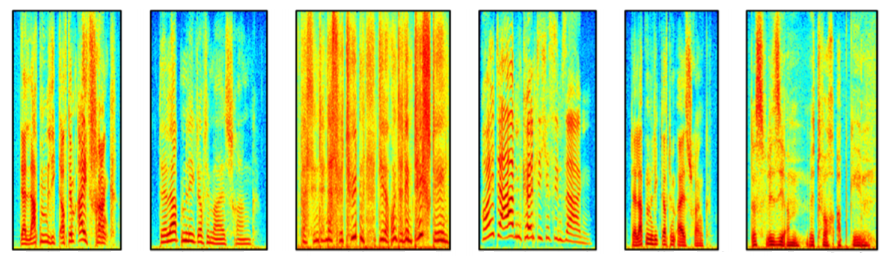
\includegraphics[width=1\textwidth]{images/spekto.PNG}
	\caption{\label{spektogram}Spektogramme für verschiedene Emotionen \cite{badshah2019deep}}
\end{figure}
\subsection{STFT und FFT}

%Bilder kann man natürlich auch in Arbeiten integrieren. Für Fotos und ähnliches %unterstützt PDF-\LaTeX{} direkt \verb|jpg| und \verb|png|, ansonsten empfiehlt es sich %Vektorgrafiken zu verwenden und diese als \verb|pdf| zu speichern. Sollte ein Bild %einmal zu viel weißen Raum um sich haben, so kann man mit dem Werkzeug \verb|pdfcrop| %das Bild automatisch ausschneiden

%\begin{figure}[ht]
%    \centering
%    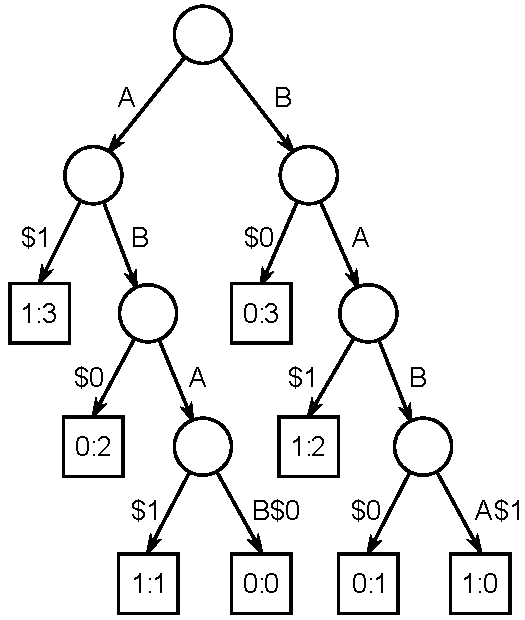
\includegraphics[width=.4\textwidth]{images/Suffix_tree_ABAB_BABA}
%    \caption{\label{anker}Bechreibung des Bilds}
%\end{figure}

%Mit Hilfe eines Labels kann man sich dann im Text auf diese Grafik (\ref{anker}) %beziehen. 

%\begin{figure}[ht]
%    \centering
%    \subfigure[Ein fettes u]{
%        
\includegraphics[width=0.2\linewidth]{images/a}
%        \label{subfigurebsp:a}
%    }
%    \hspace{1cm}
%    \subfigure[Ein dünneres u]{
%        
\includegraphics[width=0.2\linewidth]{images/b}
%        \label{subfigurebsp:b}
%    }
%    \caption{Die \emph{u}s aus der Wortmarke}
%\end{figure}

%Durch \verb|subfigure| lassen sich auch zwei kleine Bilder nebeneinander setzen. In %Abbildung \ref{subfigurebsp:a} ist ein fettes u auf der linken und in %\ref{subfigurebsp:b} ein dünneres auf der rechten Seite zu sehen.


%\subsection{Tabellen}

%Hier nur ein kurzes Beispiel, in jedem \LaTeX{} Buch finden sich gute Anleitungen zum %Erstellen von Tabellen.

%\begin{table}[h]
%    \centering
%    \begin{tabular}{|l|l|l|}
%        A & B & C \\
%        \hline
%        x & x & x \\
%        x & x & x
%    \end{tabular}
%\end{table}


%\subsection{Formeln}

%Mathematische Formeln lassen sich als Umgebung mit \verb|\begin{math}| und \verb|\end{math}| erzeugen, es gibt aber auch eine abgekürzte Schreibweise mit \verb|\( Formel \)| wobei die Formel dann im laufenden Text bleibt. Die kürzeste Form ist mit zwei \verb|$| um die Formel, z.B.~so Wasser ist H$_2$O.

%Mit der Schreibweise \verb|\[ Formel \]| wird die Formel mittig auf einer neuen Zeile gesetzt, z.B.

%\[y = x^2 \]

%Dies ist die Kurzform der Umgebung \verb|equation|, mit der die Gleichung auch nummeriert wird. 

%\begin{equation}
%    x_{1,2} = \frac{-b\pm\sqrt{b^2-4ac}}{2a}
%    \label{mitternachtsformel}
%\end{equation}

%Wenn wir z.B.~über die beliebte Mitternachtsformel (Gleichung \ref{mitternachtsformel}) schreiben wollen lässt sich diese also wie ein Bild referenzieren.




\chapter{Convolutional Neural Networks}
In den letzten Jahren haben Convolutional Neural Networks (CNN) in Zusammenhang mit Mustererkennung wie zum Beispiel Bildklassifizierung oder Spracherkennung bahnbrechende Ergebnisse erzielt \cite{bilderkennung}. Bei Bildklassifizierungen liefern CNNs die besten Ergebnisse \cite{imagenet}. Ein großer Vorteil bei CNNs ist, dass eine Reduzierung der Parameter stattfindet und dadurch größere Modelle mit komplexen Aufgaben im Anschluss besser klassifiziert werden können \cite{bilderkennung}. CNN ist ein hierarchisches neuronales Netz, welches aus unterschiedlichen Schichten (layers) besteht \cite{badshah2019deep}. Diese Schichten kann man in drei Hauptkomponenten aufteilen (siehe Abbildung \ref{architektur}.
\begin{itemize}
	\item  convolutional layers \newline diese Schicht ist für das Filtern des Inputs zuständig \cite{badshah2019deep}
	\item  pooling layers 
	\item  fully connected layers
	
\end{itemize}


\chapter{Modellarchitektur und Ablauf}

In diesem Abschnitt wird der Aufbau und die Vorgehensweise des Algorithmuses bei SER-Systemen erläutert.


\section{2 Phasen der SER}

Die große Herausforderung für SER-Systemen ist die Unterscheidung der verschiedenen Emotionen durch die Sprache zu ermöglichen. Jeder Sprecher hat individuelle und kulturell bedingte Sprechstile, Sprechgeschwindigkeit, unterschiedliche Tonhöhe und Energiekontur im Spektrogramm, was das Extrahieren der Merkmale erschwert \cite{badshah2019deep}. Diese Umstände werden in der Verarbeitungseinheit behandelt, um später beim Klassifizieren der Sprachsignale gute Ergebnisse zu erhalten. 
\subsection{Verarbeitungseinheit (processing unit)}
Um die in 3.1 genannten Probleme anzugehen wird in der Verarbeitungseinheit das Spektrogramm in mehrere Blöcke (chunks) aufgeteilt, die Frames genannt werden (siehe Abbildung \ref{frames}) \cite{badshah2019deep}.
\begin{figure}[ht]
	\centering
	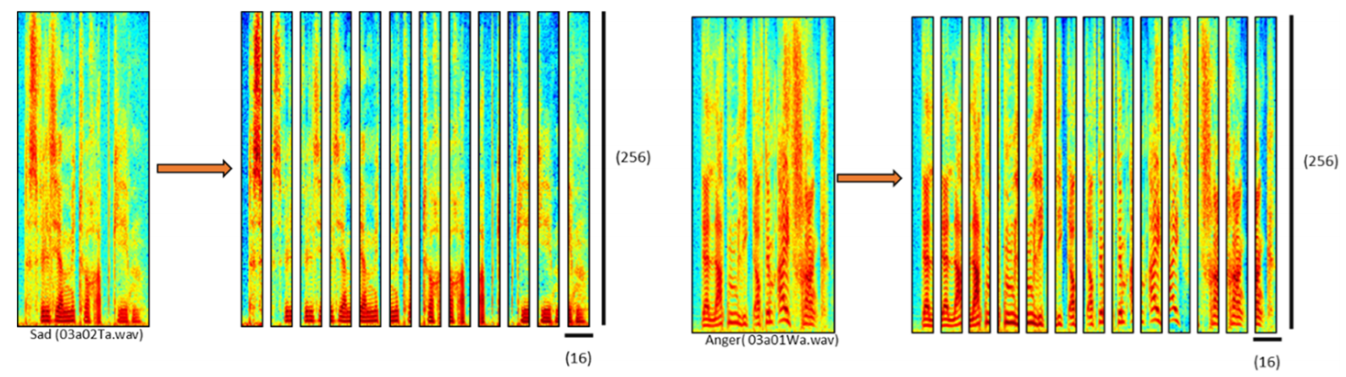
\includegraphics[width=1\textwidth]{images/frames}
	\caption{\label{frames} in Frames ausgeteilte Spektrogramme \cite{badshah2019deep}}
\end{figure}
\subsection{Klassifikator (classifier)}
Nachdem das Spektrogramm in mehreren Frames aufgeteilt wurde findet die Klassifikation mit Hilfe von Machine Learning Algorithmen statt \cite{badshah2019deep}. Hierbei werden die Frames einzeln untersucht und es kommen verschiedene Arten von Klassifikatoren zum Einsatz. Die gängigsten Algorithmen sind Hidden-Markov-Modelle (HMM), Gaußsches Mischungsmodell, Support Vector Machine (SVM), künstliche neuronale Netze und K-nearest neighbor, wobei SVM und HMM die am weitesten verbreiteten Lernalgorithmen für sprachbezogene Anwendungen sind \cite{badshah2019deep}.

\section{Aufbau der Modellarchitektur}


\begin{figure}[ht]
    \centering
    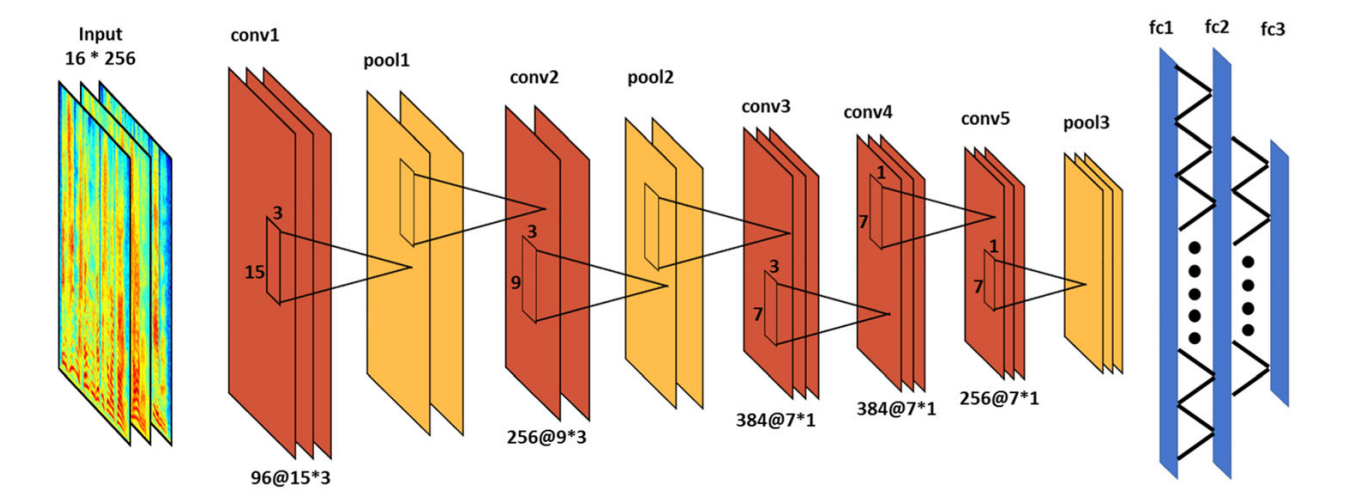
\includegraphics[width=1\textwidth]{images/conv}
    \caption{\label{architektur}CNN Architektur mit den unterschiedlichen Schichten \cite{badshah2019deep}}
\end{figure}

Mit Hilfe eines Labels kann man sich dann im Text auf diese Grafik (\ref{architektur}) beziehen. 



\section{Der Ablauf bei SER}

\begin{figure}[ht]
	\centering
	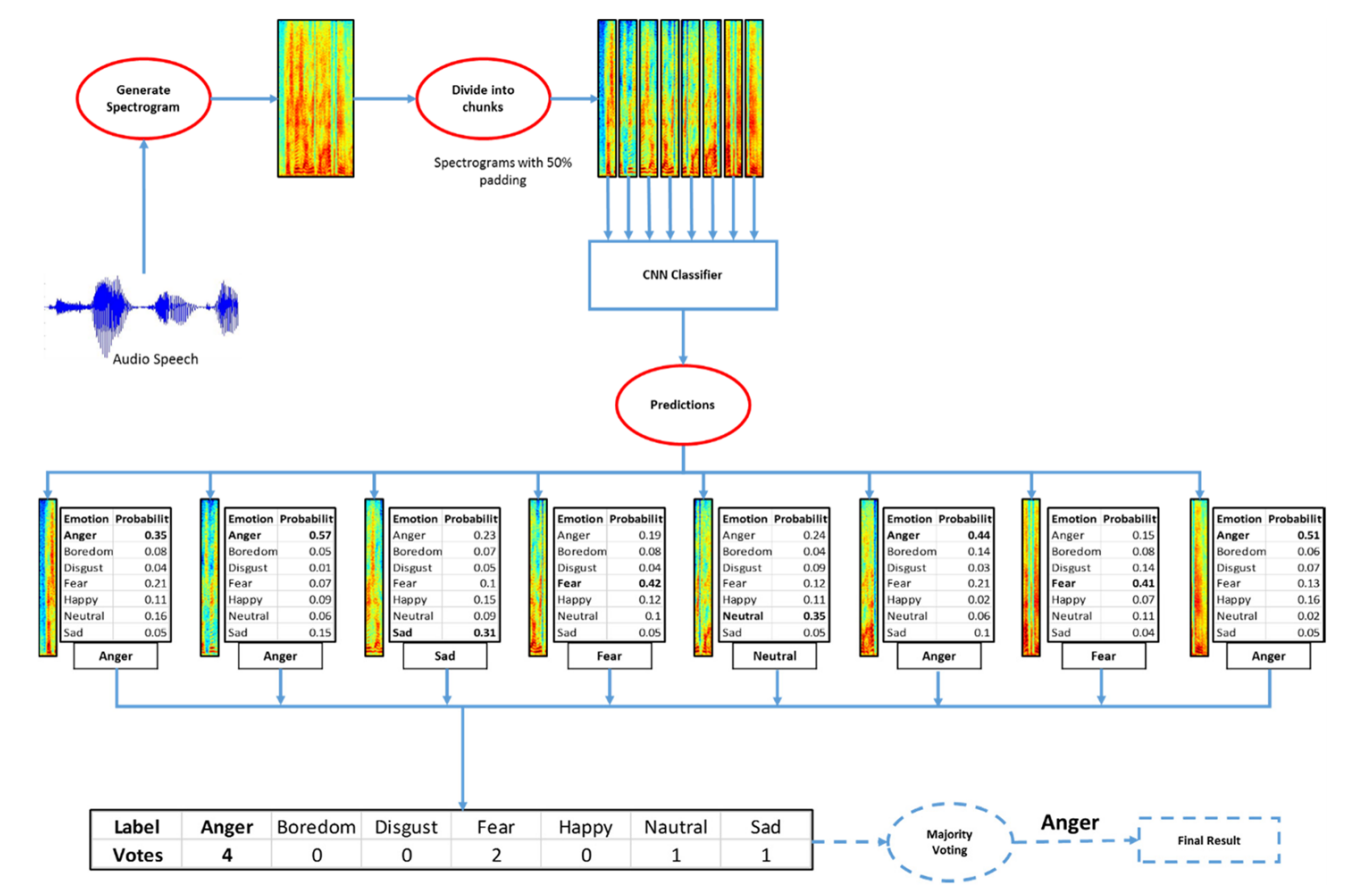
\includegraphics[width=1\textwidth]{images/ablauf}
	\caption{\label{ablauf}spezifischer Schema und Ablauf bei SER \cite{badshah2019deep}}
\end{figure}





\chapter{Schlussfolgerung}

SER bietet ein breites Spektrum an Einsatzmöglichkeiten an und die Anwendungen von diesen Spracherkennungssystemen nehmen rasant zu. In der Automobilbranche kann eine Einsatzmöglichkeit, um den mentalen Zustand des Fahrers zu tracken, stattfinden \cite{badshah2019deep}. Des weiteren kann SER eine wichtige Komponente bei der Entwicklung intelligenter Dienste in der Gesundheitversorgung, Audio-Forensik und Mensch-Maschine Interaktion sein \cite{badshah2019deep}.

% hier weitere Kapitel einbinden


%%
%% Anhänge
%%
\appendix
\chapter{Quelltexte}

In diesem Anhang sind einige wichtige Quelltexte aufgeführt.

\begin{lstlisting}
public class Hello {
    public static void main(String[] args) {
        System.out.println("Hello World");
    }
}
\end{lstlisting}



%%
%% Nachspann
%%
\backmatter


%%
%% Literaturverzeichnis
%%
\bibliography{bibliography}


%%
%% Versicherung
%%
\cleardoublepage
\thispagestyle{empty}

Name: \fullname \hfill Matrikelnummer: \matnr \vspace{2cm}

\minisec{Erklärung}

Ich erkläre, dass ich die Arbeit selbständig verfasst und keine anderen als die angegebenen Quellen und Hilfsmittel verwendet habe.\vspace{2cm}

Ulm, den \dotfill

\hfill {\footnotesize \fullname}
\end{document}
